% Part: biographies 
% Chapter: alan-turing 
% Section: biography 
\documentclass[../../../include/open-logic-section]{subfiles}

\begin{document}

\olfileid{bio}{alt}{bio} 
\olsection{Biography}
\begin{figure}[h!] 
\centering 
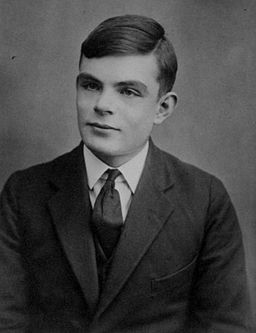
\includegraphics[scale=0.75]{alan-turing.jpg}
\caption{Alan Turing. Photo Credit: Wikimedia Commons.} 
\end{figure}

Alan Turing was born in Mailda Vale, London, on June 23, 1912. He is
considered the father of theoretical computer science. Turing's interest in
the physical sciences and mathematics started at a young age. However, as a
boy his interests were not represented well in his schools, where emphasis
was placed on literature and classics. As such, he did poorly in school and
was reprimanded by many of his teachers.

Turing attended King's College, Cambridge as an undergraduate, where he
studied mathematics. In 1936 Turing developed (what is now called) the
Turing machine as an attempt to precisely define the notion of a computable
functon. He was beaten to the result by Alonzo Church, with the development
of the lambda calculus, though Turing's paper was still published with
reference to Church's result. He spent 1936 to 1938 in Princeton studying
under Church, where he obtained his doctorate.

Despite his interest in Logic, Turing's earlier interests in physical
sciences remained prevalent. His practical skills were put to work when he
became employed full time with the British cryptanalytic department at
Bletchley Park during World War II. Turing was a central figure in cracking
the cypher used by German Naval communications - the Enigma code. 
 Turing's expertise in statistics and cryptography, and the introduction of electronic
machinery gave the team the ability to crack the code by creating a 
de-crypting machine called ``bombe". His ideas also helped in the creation
of the world's first programmable electronic computer, the Colossus.

Turing never married, as he identified as a homosexual. However, in 1942 he
proposed to Joan Clarke, one of his teammates at Bletchley Park, but
revoked the proposal and confessed to her that he was homosexual
\citep[259]{Hodges2014}. He had several lovers throughout his lifetime,
although homosexual acts were considered criminal offences in the UK. In
1952 Turing's house was burgled by a friend of his lover at the time, and
during a police report he admitted to having a sexual relationship with the
man, under the impression that the government was on their way to
legalizing homosexual acts \citep[575]{Hodges2014}. This was not true, and
he was charged with gross indecency \citep[576]{Hodges2014}. Instead of
going to prison, Turing opted for a hormone treatment that reduced libido.
Turing was found dead on June 8, 1954, of a cyanide overdose - most likely
suicide.

\begin{reading}
\begin{itemize} 
\item For a comprehensive biography of
Alan Turing, which also served as the inspiration behind \emph{The
Imitation Game}, see \citet{Hodges2014}.

\item \emph{The Imitation Game}, an Academy Award nominated film starring
Bendict Cumberbatch and Kiera Knightley, is loosely based off of Alan
Turing’s life and time at Bletchley Park. See \citet{Imitation2014}.

\item For a podcast on the life of Alan Turing, see \citet{Radiolab2012}. A
related podcast on the Turing test is available at \citet{RadiolabND}.

\item Turing's original presentation of the Turing machine can be found at
\citet{Turing1937}.

\item BBC Horizon's documentary \emph{The Strange Life and Death of Dr. 
Turing} is available to watch online. See \citet{Sykes1992}.

\item Check out this short video of a working LEGO Turing Machine -
made to honour Turing's centenary in 2012 \citep{Theelen2012}.

\end{itemize}

\end{reading}

\end{document}
